\chapter{GEM Detector Data Analysis}
Gas Electron Multiplier (GEM) detector technology invented by F.~Sauli~\cite{Sauli} in 1997 allows  high resolution track reconstruction under high rate conditions over a large area.  At the heart of these detectors is a 50 $\mu$m polyamide foil, sandwitched between two layers of 5 µm copper.  This foil is punctured with 70 µm circular holes in a regular hexagonal pattern, spaced 140 µm apart. The GEM detector  features a cathode on top, while a readout board is situated  at the bottom of the detector  for collecting the electrons generated during the ionization process. The space between the cathode and the readout is occupied by three GEM foils 
 in a triple GEM detector. The 3 mm gap between the cathode and the top GEM foils forms the primary  ionization region of the detector. When a high energy particles travels through the detector it produces a trail of ionization in this region. The electrons created in this ionization drift down towards the readout layer through the GEM holes. When a potential difference of about  350 V is applied between the two layers of copper on either side of the polyamide layers of a GEM foil,    a strong  electric field is created  within the holes.  The electrons accerating in this field create secondary ionizations  resulting  in an electron avalanche. This avalanche electron travels along the electric field and are  eventually collected by the finely spaced strips of the readout layer. To enhance the amplification, multiple GEM detector layers are stacked together, allowing ionized electrons to be amplified multiple times before reaching the readout board.

The GEM detectors utilized in the PRex/CRex experiment were  designed  and built for Jefferson Lab Super BigBite Spectrometer (SBS) {\bf NL: add a reference} and span an active area of 50 cm x 60 cm each.  The PRex/CRex experiment offered an excellent opportunity to test the GEM detector in a real experimental environment before initiating the SBS experiment. PRex/CRex experiments benifited from this because the GEM detectors served as a valuable supplement to the existing detectors in situations where the event rate is very high, as the VDC efficiency declines or even fails under such conditions. This chapter delves into the apparatus and the analysis results of the GEM detectors.

\section{GEM Detector Configuration}

The SBS GEM detector used in the PRex/CRex experiment comprises three layers of GEM foils. The cathode, situated on top of the GEM foil, features a similar hole structure but is single-side coated instead of double-sided. To prevent polarization due to charge accumulation on the cathode, a thin aluminized gas window layer is applied, which shares the same high voltage as the cathode.

A premixed gas containing $75\%$ Argon and $25\%$ Carbon Dioxide is supplied by the Hall A gas system for use in the GEM detector. This mixed gas first enters the chamber between the entrance window and the cathode, then passes through the holes in the foil, ensuring a uniform gas mixture throughout the entire chamber. Exhaust gas exits through exhaust holes located on the frame at the bottom of the GEM chamber.

At the base of the GEM foils, avalanche electrons are collected by 2D readout strips. Each readout strip is connected to a charge-sensitive pre-amplifier electronics channel. To counteract any bending of the readout board due to the mixed gas in the chamber, an additional chamber is designed beneath the readout board and filled with air at the same pressure as the GEM chambers.


\begin{figure}[!tbp]
  \centering
  \begin{minipage}[b]{0.45\textwidth}
    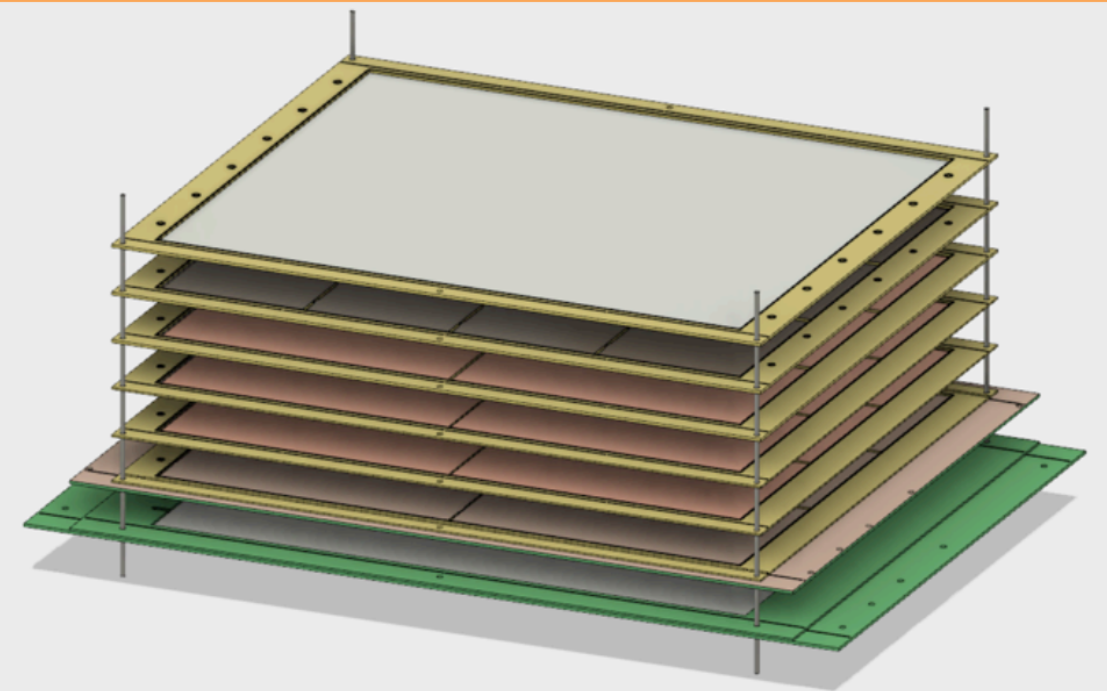
\includegraphics[width=\textwidth]{images/chap5/gem_structure_3d.png}
    \caption{GEM Chamber 2D structure}
  \end{minipage}
  \hfill
  \begin{minipage}[b]{0.45\textwidth}
    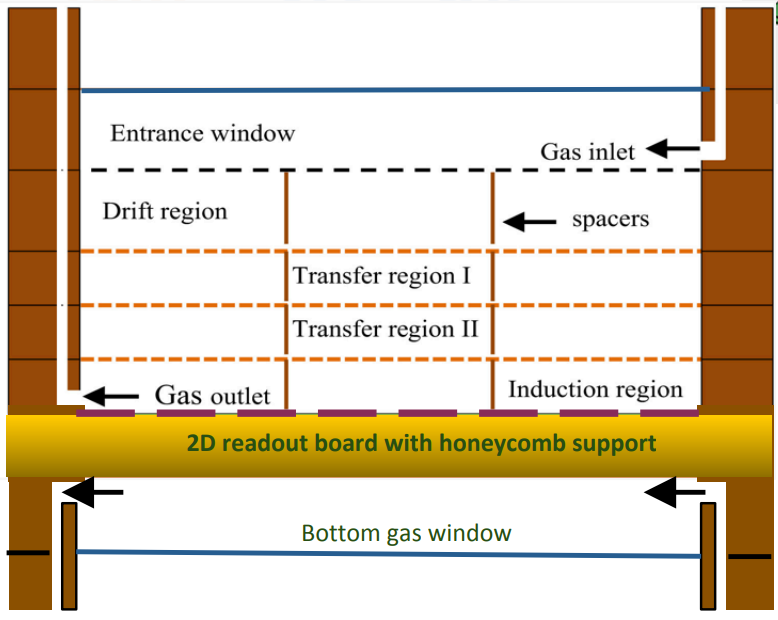
\includegraphics[width=\textwidth]{images/chap5/gem_structure_chamber_2d.png}
    \caption{GEM chamber Gas flow}
  \end{minipage}
\end{figure}


\subsection{GEM Detector in Hall A High-Resolution Spectrometer}

Each High-Resolution Spectrometer (HRS) in Hall A is equipped with three large SBS GEM detectors, each measuring $50 cm \times 60 cm$, and three smaller GEM detectors measuring $10 cm \times 20 cm$ produced by Idaho State University. As depicted in the corresponding figure, the GEM detectors are arranged parallel to each other and placed after the Vertical Drift Chamber (VDC) detectors. The smaller Idaho GEM detectors are positioned in front of the larger SBS GEM detectors. Two quartz detectors are placed between the first and second Idaho GEM detectors, while two AT detectors are situated between the SBS GEM detectors and the Idaho GEM detectors.


\begin{figure}[!htbp]
  \centering
  \begin{minipage}[b]{0.45\textwidth}
    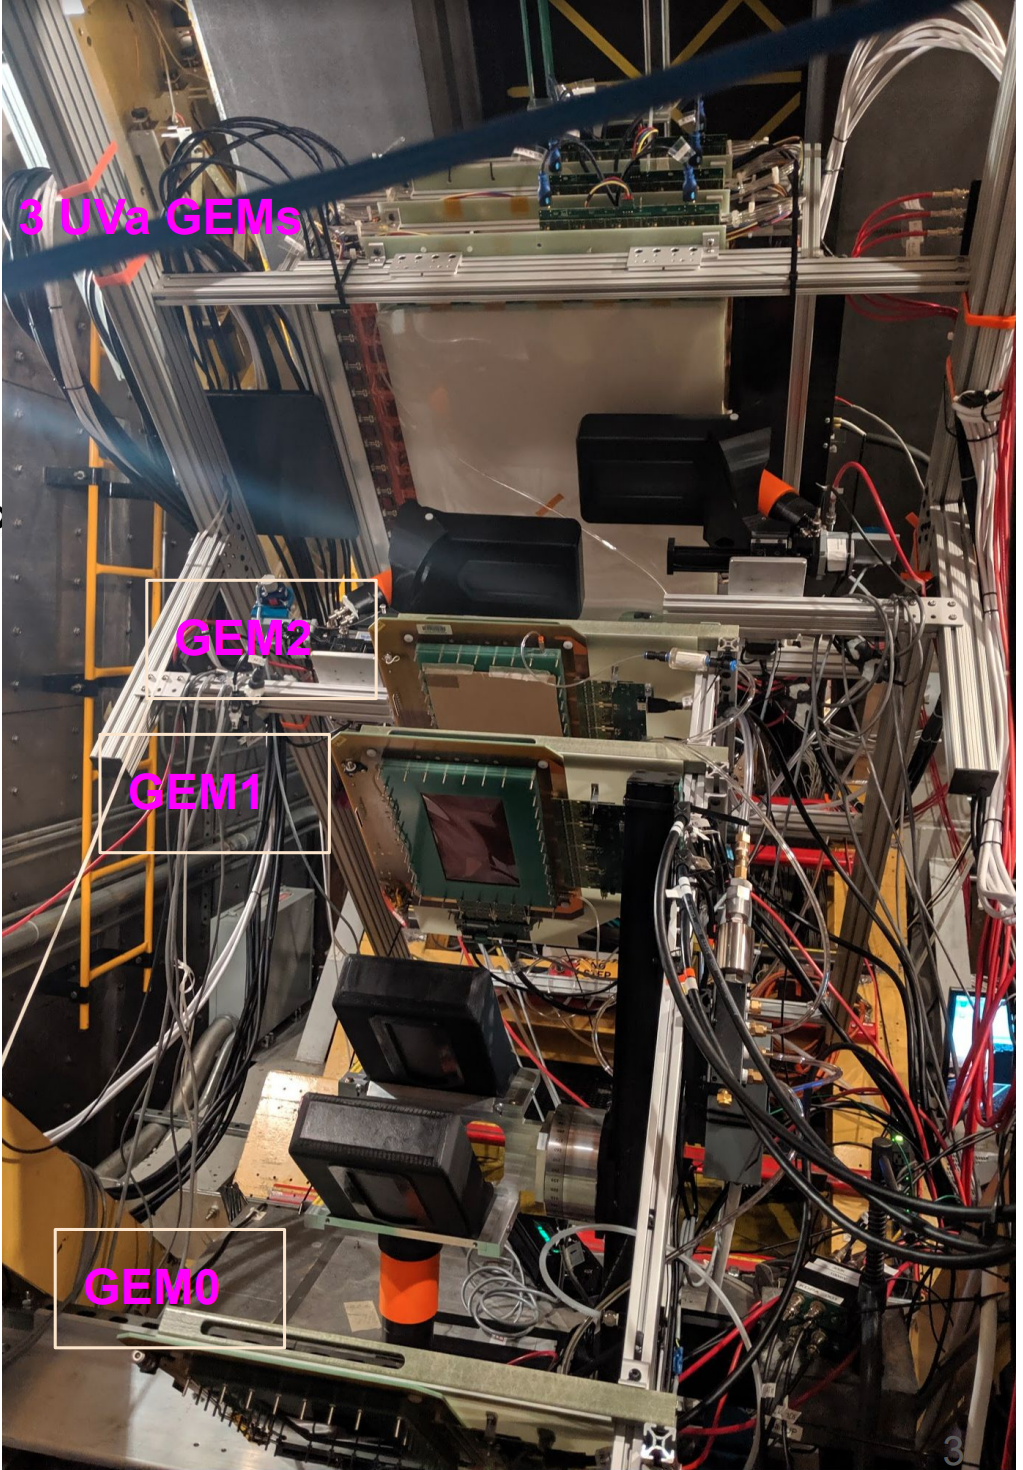
\includegraphics[width=\textwidth]{images/chap5/gem_in_apparatus_photo.png}
    \caption{GEM Chamber 2D structure}
  \end{minipage}
  \hfill
  \begin{minipage}[b]{0.45\textwidth}
    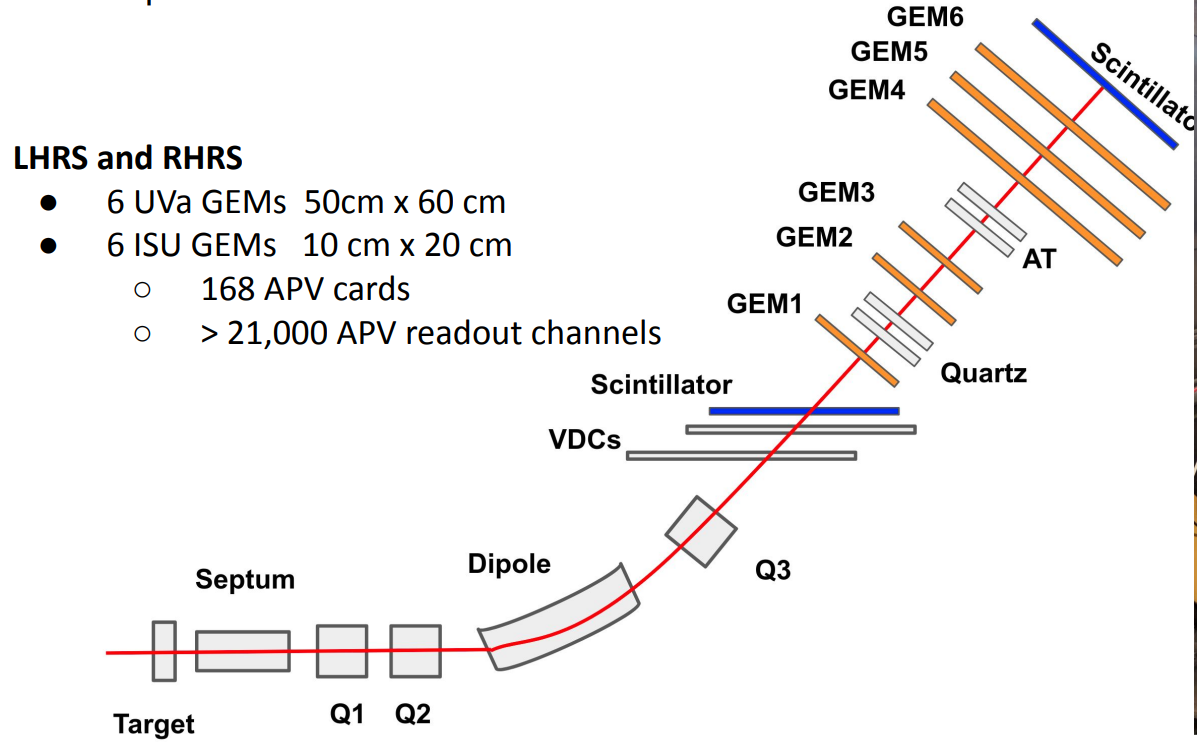
\includegraphics[width=\textwidth]{images/chap5/gem_apparatus_in_hrs_2d.png}
    \caption{GEM chamber Gas flow}
  \end{minipage}
\end{figure}


\subsection{Add a more detailed introduction of GEM detector supplement electronics??}
\begin{enumerate}
    \item readout electronics (APV, MPD, CPU, coda)
    \item low voltage for the APV (modular LV, cable selection, LV regulator, cooling fan) 
    \item High Voltage
    \item Gas System
\end{enumerate}


\begin{figure}[!htbp]
  \centering
  \begin{minipage}[b]{0.45\textwidth}
    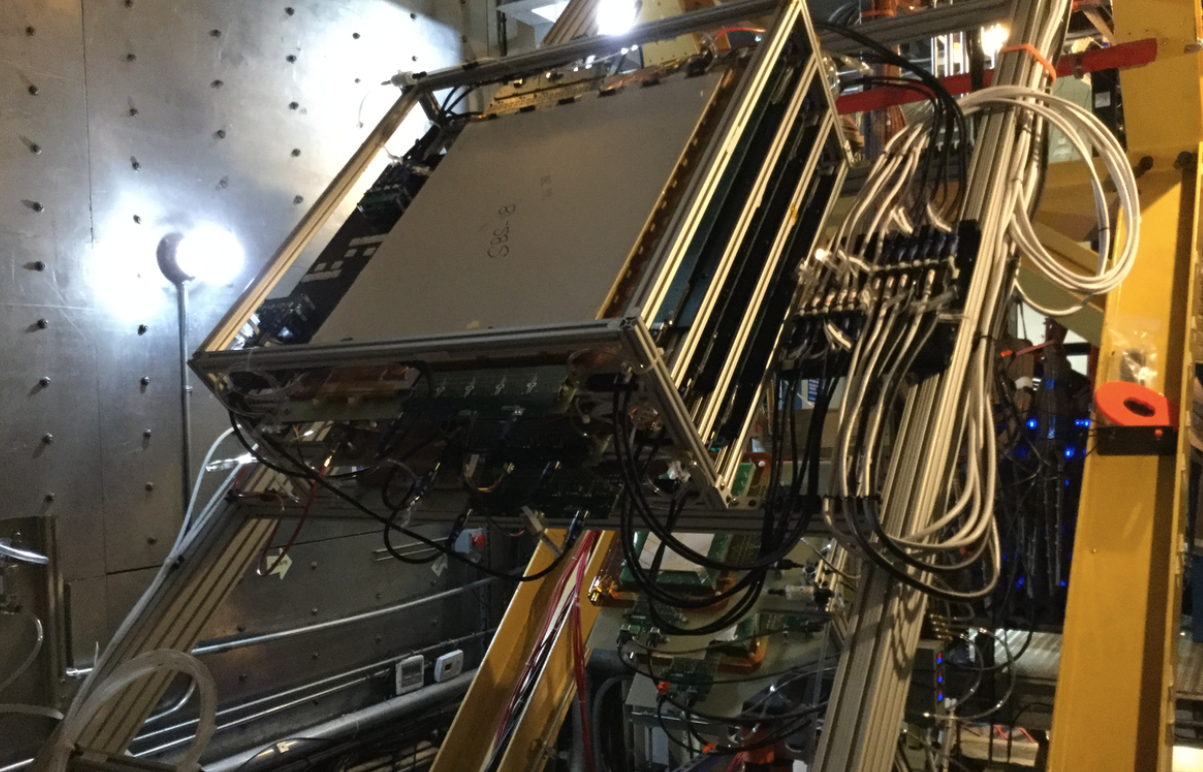
\includegraphics[width=\textwidth]{images/chap5/gem_in_hrs.png}
    \caption{GEM Chamber in HRS}
  \end{minipage}
  \hfill
  \begin{minipage}[b]{0.45\textwidth}
    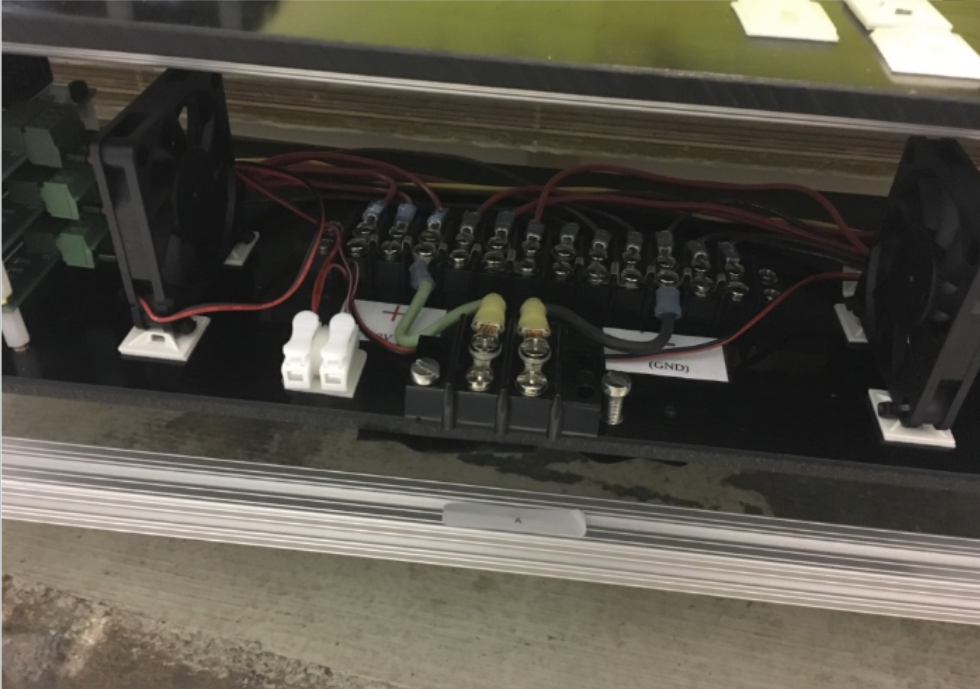
\includegraphics[width=\textwidth]{images/chap5/gem_low_voltage.png}
    \caption{GEM Pre-Amplifier Voltage Supply}
  \end{minipage}
\end{figure}


\begin{figure}
    \centering
    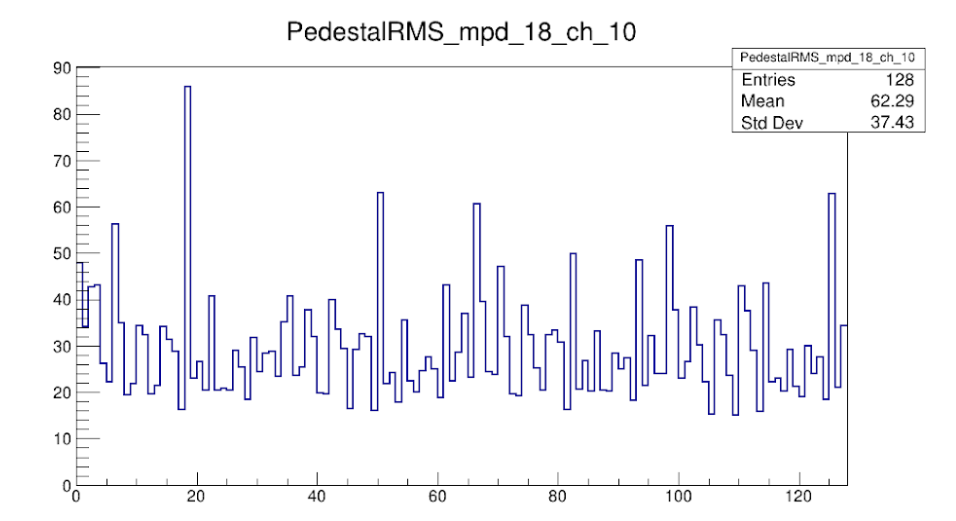
\includegraphics[width=\textwidth]{images/chap5/gem_signal.png}
    \caption{Caption}
    \label{fig:apv_25_pedestal_plot}
\end{figure}

\section{GEM Detector Data Analysis}

The GEM detector readout strips are connected to the APV frontend card, a 128-channel pre-amplifier. The signal from the APV is transmitted to a Multi-Purpose Digitizer, where it is converted to digital signals using a 12-bit Analog to Digital Converter. Figure \ref{fig:apv_25_pedestal_plot} displays a typical plot after MPD conversion. The x-axis represents the APV channels, and the y-axis corresponds to the ADC values after the conversion, which are proportional to the number of charges collected by the given strip.

To extract useful signals, multiple steps are typically employed, including common mode subtraction, pedestal measurement, and fired strips selection.

\subsection{GEM Pedestal Measurement}

A pedestal run involves setting the high voltage to 2000 V for a dry run. At this high voltage, the electric field is insufficient to trigger an avalanche, meaning no signal should be detected on the readout strips. By applying a 2000 V high voltage, the noise from the high voltage modules can be considered when estimating the pedestal, as opposed to having no high voltage applied. The pedestal of each channel of the 128 APV channels is calculated by subtracting the ADC value from the common mode, defined as the average of the 128-channel ADC values. Subsequently, the Root Mean Square (RMS) and mean of each channel's pedestal are computed across all the events that have been recorded.

Figure \ref{fig:lhrs_pedestal_distribution} and \ref{fig:rhrs_pedestal_distribution} show the pedestal distributions of all the channels used in the PRex experiment. The x-axis represents the index of the APV card, and the y-axis corresponds to the RMS value of the pedestal. Each data point in the plot represents one GEM readout channel.

The first 18 APV cards are utilized in the Idaho GEM detectors. As the area of these detectors is $10 cm \times 20 cm$, their pedestal RMS values are also smaller than those of the SBS GEM detectors. The LHRS GEM detectors have larger pedestal RMS values than those of the RHRS, with RMS values of around 20 ADC, which equates to approximately $0.02 V$ voltage fluctuation. A few channels in each APV card exhibit much higher pedestals, and these are considered dead channels due to issues in the Printed Circuit Board (PCB) manufacturing process.

\begin{figure}[!htbp]
    \centering
    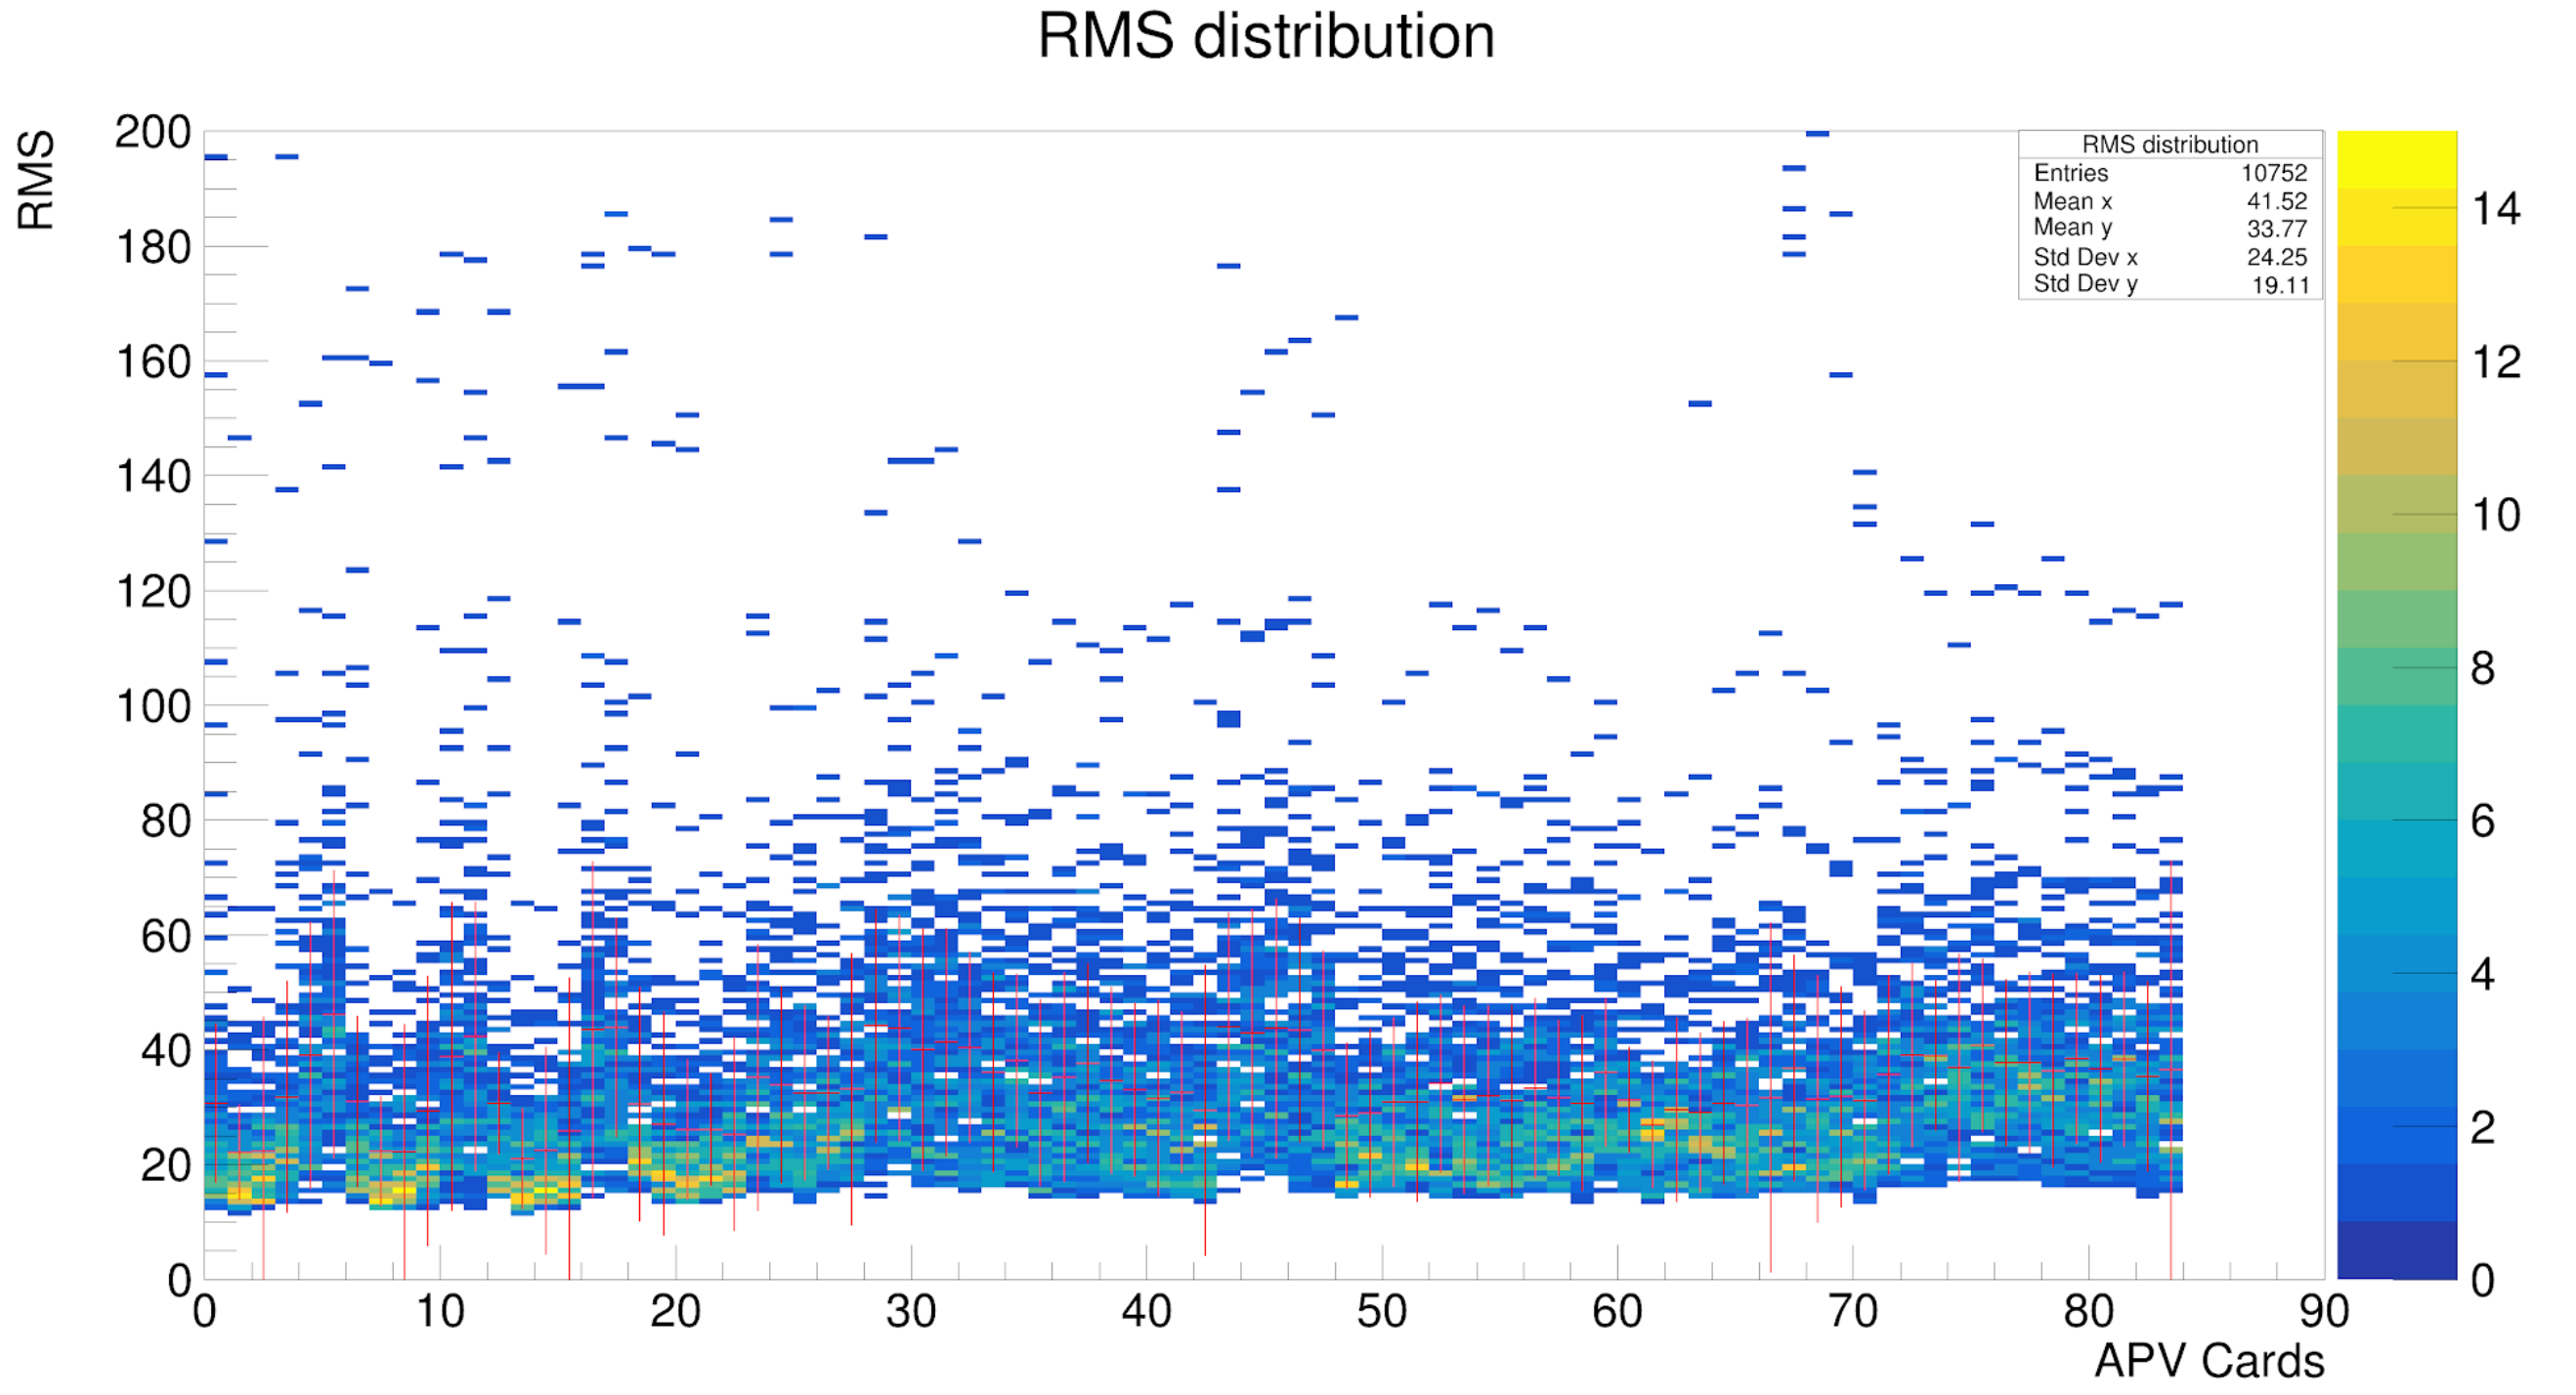
\includegraphics[width=\textwidth]{images/chap5/LHRS_pedestal.png}
    \caption{LHRS GEM Readout RMS of Pedestal Distribution}
    \label{fig:lhrs_pedestal_distribution}
\end{figure}

\begin{figure}[!htbp]
    \centering
    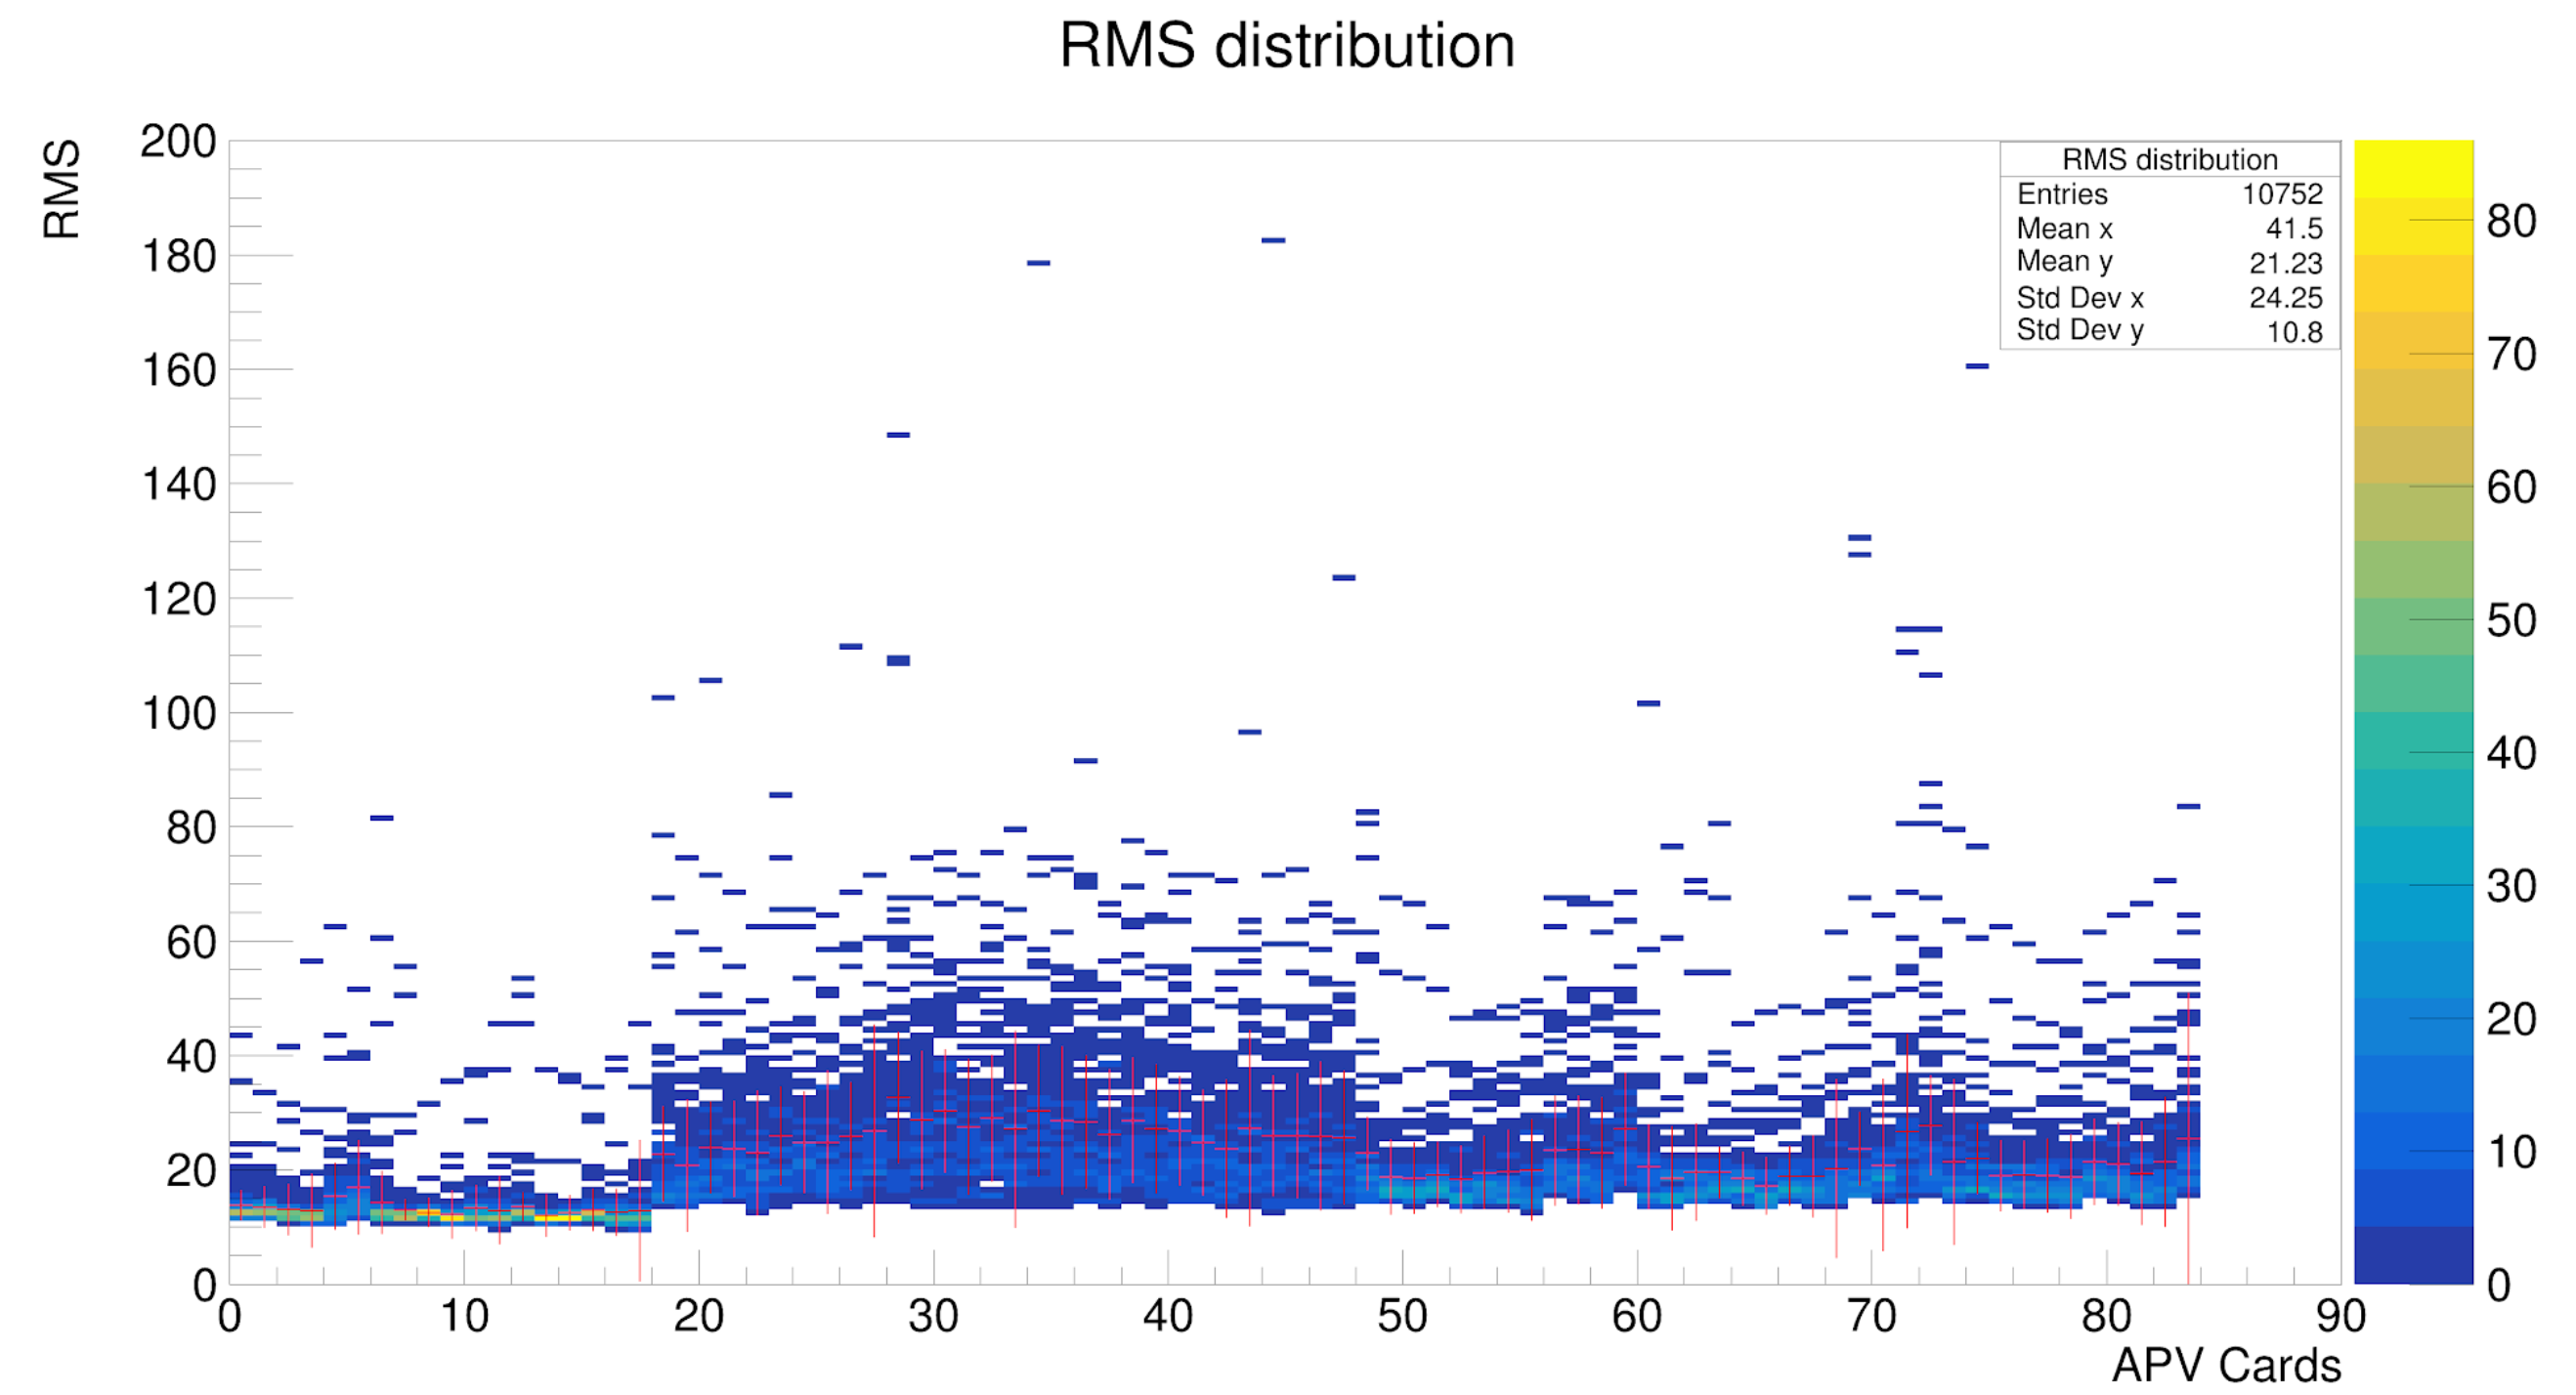
\includegraphics[width=\textwidth]{images/chap5/rhrs_pedestal.png}
    \caption{RHRS GEM Readout RMS of Pedestal Distribution}
    \label{fig:rhrs_pedestal_distribution}
\end{figure}


\subsubsection{GEM detector false positive rate}

When the GEM detector works at Normal working voltage. When a particle passes through  
the GEM detectors and ionized the gases inside the GEM chambers. The ionized electrons 
will travel along the Electric field and get amplified within the holes in GEM detectors, 
and then the avalanche electrons will be collected by the readout strips and readout with the electronics. 

The common mode correction of raw signal ADC values is done using the same algorightm as
 in the case of pedestal ADCs. After that, the pedestal corrected ADC value for each strip is
calculated by  subtracting  the mean of the pedestal for that strip from the common mode 
corrected ADC value. The determination of fired  GEM  strips is achieved  
by comparing the corrected ADC  values with the pedestal thresholds. Different channels may have different 
noise performances, for example,  due to different strip capacitances.  To get a consistent criterion,
 the threshold for a  given channel is chosen to be N $\times$ (RMS of the pedestal).  
If the value is larger than the threshold, then the  given strip is  considered to have fired,
 and the strip number along with  its corrected ADC value are written into the fired strip array.  
If the corrected ADC value is lower than the threshold, then the correctd ADC value for that strip 
is set to zero, and the strip is marked as non-fired. The constant N was typically set to 5 for 
SBS GEM modules used in PRex/CRex exeperiments. 

Setting the threshold   too high with a high value of N increases the probability of  actualy  fired 
good signal  strips to  be categorized as  non-signal  (False Negative), leading to artificial reduction 
of detection efficiency.  On the other hand, if the threshold is set too low, it increases the the 
 chance that pedestal  noise is categorized as good signals from fired strips (False Positive). 

To measure the false positive rate, the GEM signal selection algorithm was applied on a 2000 V voltage 
dry run, other than the dry run used for the pedestal calculation. Since there are no real signals  at 
2000 V,  any fired strips in this run are false positive signals. By measuring the ratio of the fired 
strips in the dry run total number of triggers, we can estimate the False Positive Rate of the algorithm. 
In fig \ref{fig:lhrs_fake_hit_rate} and \ref{fig:rhrs_fake_hit_rate} are the false positive  hit rate 
for the SBS GEM detectors on LHRS and RHRS. At the $5\sigma$ threshold, the false hit rate for LHRS 
was $0.16\%$ and $0.01\%$.

\subsubsection{High Voltage Scan Efficiency for GEM detectors}
\subsubsection{GEM detector number of cluster performance}
\subsubsection{GEM detector cluster size performance}


\begin{figure}[!htbp]
    \centering
    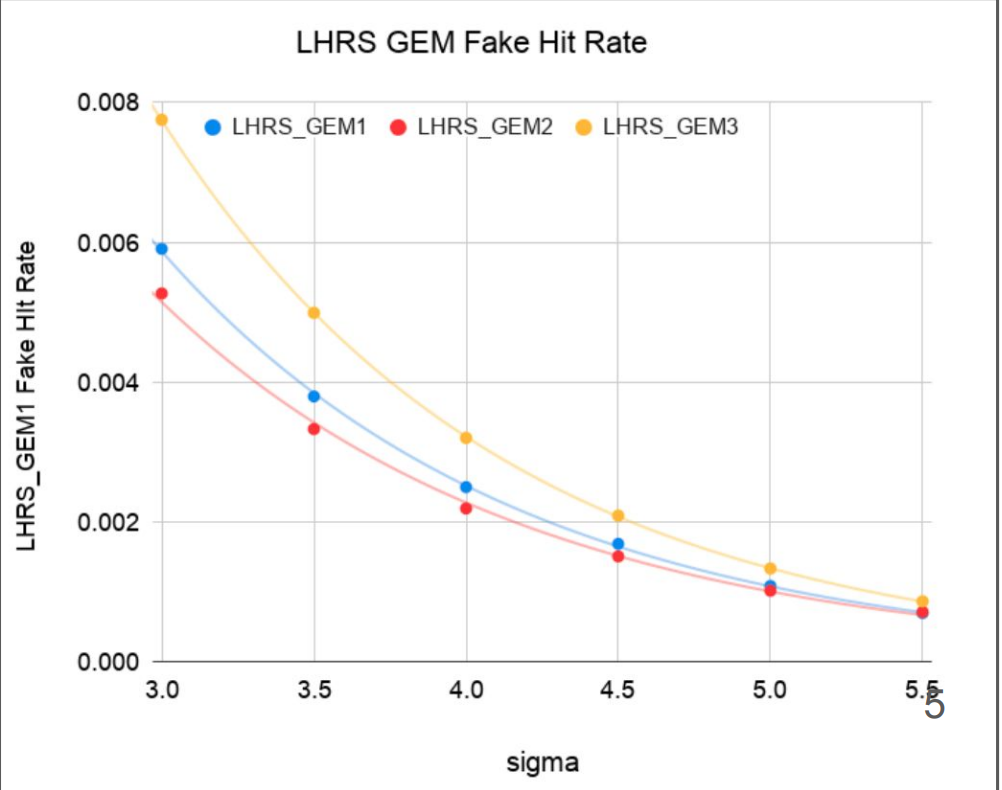
\includegraphics[width=\textwidth]{images/chap5/lhrs_fake_hit_rate.png}
    \caption{LHRS SBS GEM Fake Hit Rate}
    \label{fig:lhrs_fake_hit_rate}
\end{figure}

\begin{figure}[!htbp]
    \centering
    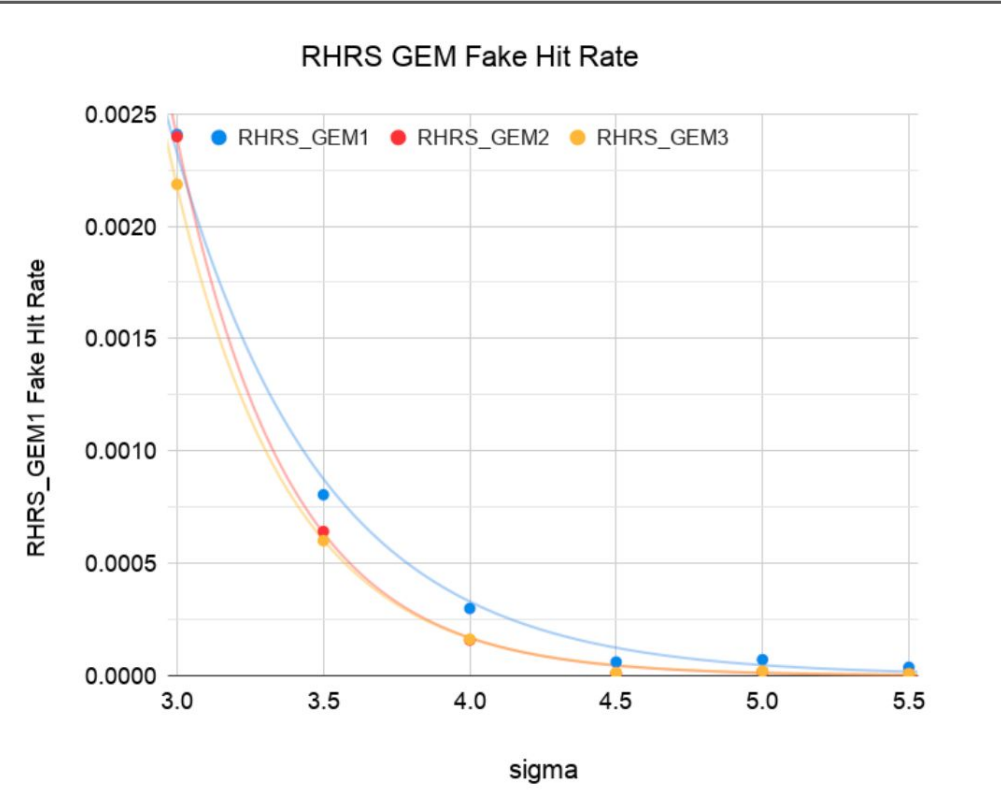
\includegraphics[width=\textwidth]{images/chap5/rhrs_fake_hit_rate.png}
    \caption{RHRS SBS GEM Fake Hit Rate}
    \label{fig:rhrs_fake_hit_rate}
\end{figure}

\subsection{GEM detector alignment}

\subsubsection{tree search algorithm used for search for the GEM cluster}
\subsubsection{Multiple GEM detectors alignment algorithm }
\subsection{GEM detector performance}

The GEM detectors in the spectrometer serve as an excellent supplement to the VDC detector employed for tracking scattered electrons. The efficiency of the detector is crucial for its performance. Both the VDC and GEM detectors can provide scattered electron tracks, enabling us to use the reconstructed track of the scattered electrons to project the track onto a given detector and measure the GEM detector's efficiency.

The GEM foil is a two-layer copper-coated structure, with avalanches occurring only inside the holes of the GEM foil. Ionized ions are absorbed by the copper layers, reducing the travel distance to at most 70 µm. This is a significant reduction compared to the drift chamber, which is limited in its maximum event rate due to drift time. The maximum working rate for the drift chamber is limited to approximately 100 kHz, whereas the GEM detector's event rate can reach MHz per square centimeter. In this section, we will discuss the detailed measurement of GEM efficiency using the tracking method and compare the high-rate performance of the GEM and VDC detectors.

\subsubsection{GEM Detector Efficiency with Tracking}

Each HRS has four layers of VDC chambers, providing highly accurate position and angular information for 
the track. Taking the VDC as a reference, we project the track reconstructed from the VDC plane 
onto each GEM detector. We then search for events within a $4 cm \times 4 cm$ area 
(justify the choice of a 4x4 area instead of a smaller one). 

{\bf NL: Good point: you can do this by calculating the mutiple scattering angle on the top windows, 
the thick protective aluminum shield on top of the VDC stack, quartz detectors etc. Then use this angle
 and the distance to GEM to estimate the error in the projection. You can do more pricisely by doing a 
small simulation instead of using one distance}

If a good GEM hit is present within the search area, then that event  is considered  efficient; if not,
 inefficient. Figures \ref{fig:lhrs_efficiency_2d} and \ref{fig:rhrs_efficiency_2d} show  the position 
dependent  GEM detector efficiency for LHRS and RHRS, respectively, for a typical PRex GEM run.

\begin{table}[]
    \centering
    \begin{tabular}{c|c|c|c|c|c|c} \hline
         ~ & GEM 1 & GEM 2 & GEM 3 & GEM 1 & GEM 2 & GEM 3 \\ \hline 
         RHRS & $96\%$ & $96\%$ & $96\%$ & $92\%$& $92\%$& $92\%$  \\ \hline
         LHRS & $86\%$& $84\%$ & $87\%$ & $88\%$ & $66\%$ & $92\%$ \\ \hline
    \end{tabular}
    \caption{GEM Detector efficiency}
    \label{tab:gem_detector_efficiency_table}
\end{table}

\begin{figure}[!htbp]
    \centering
    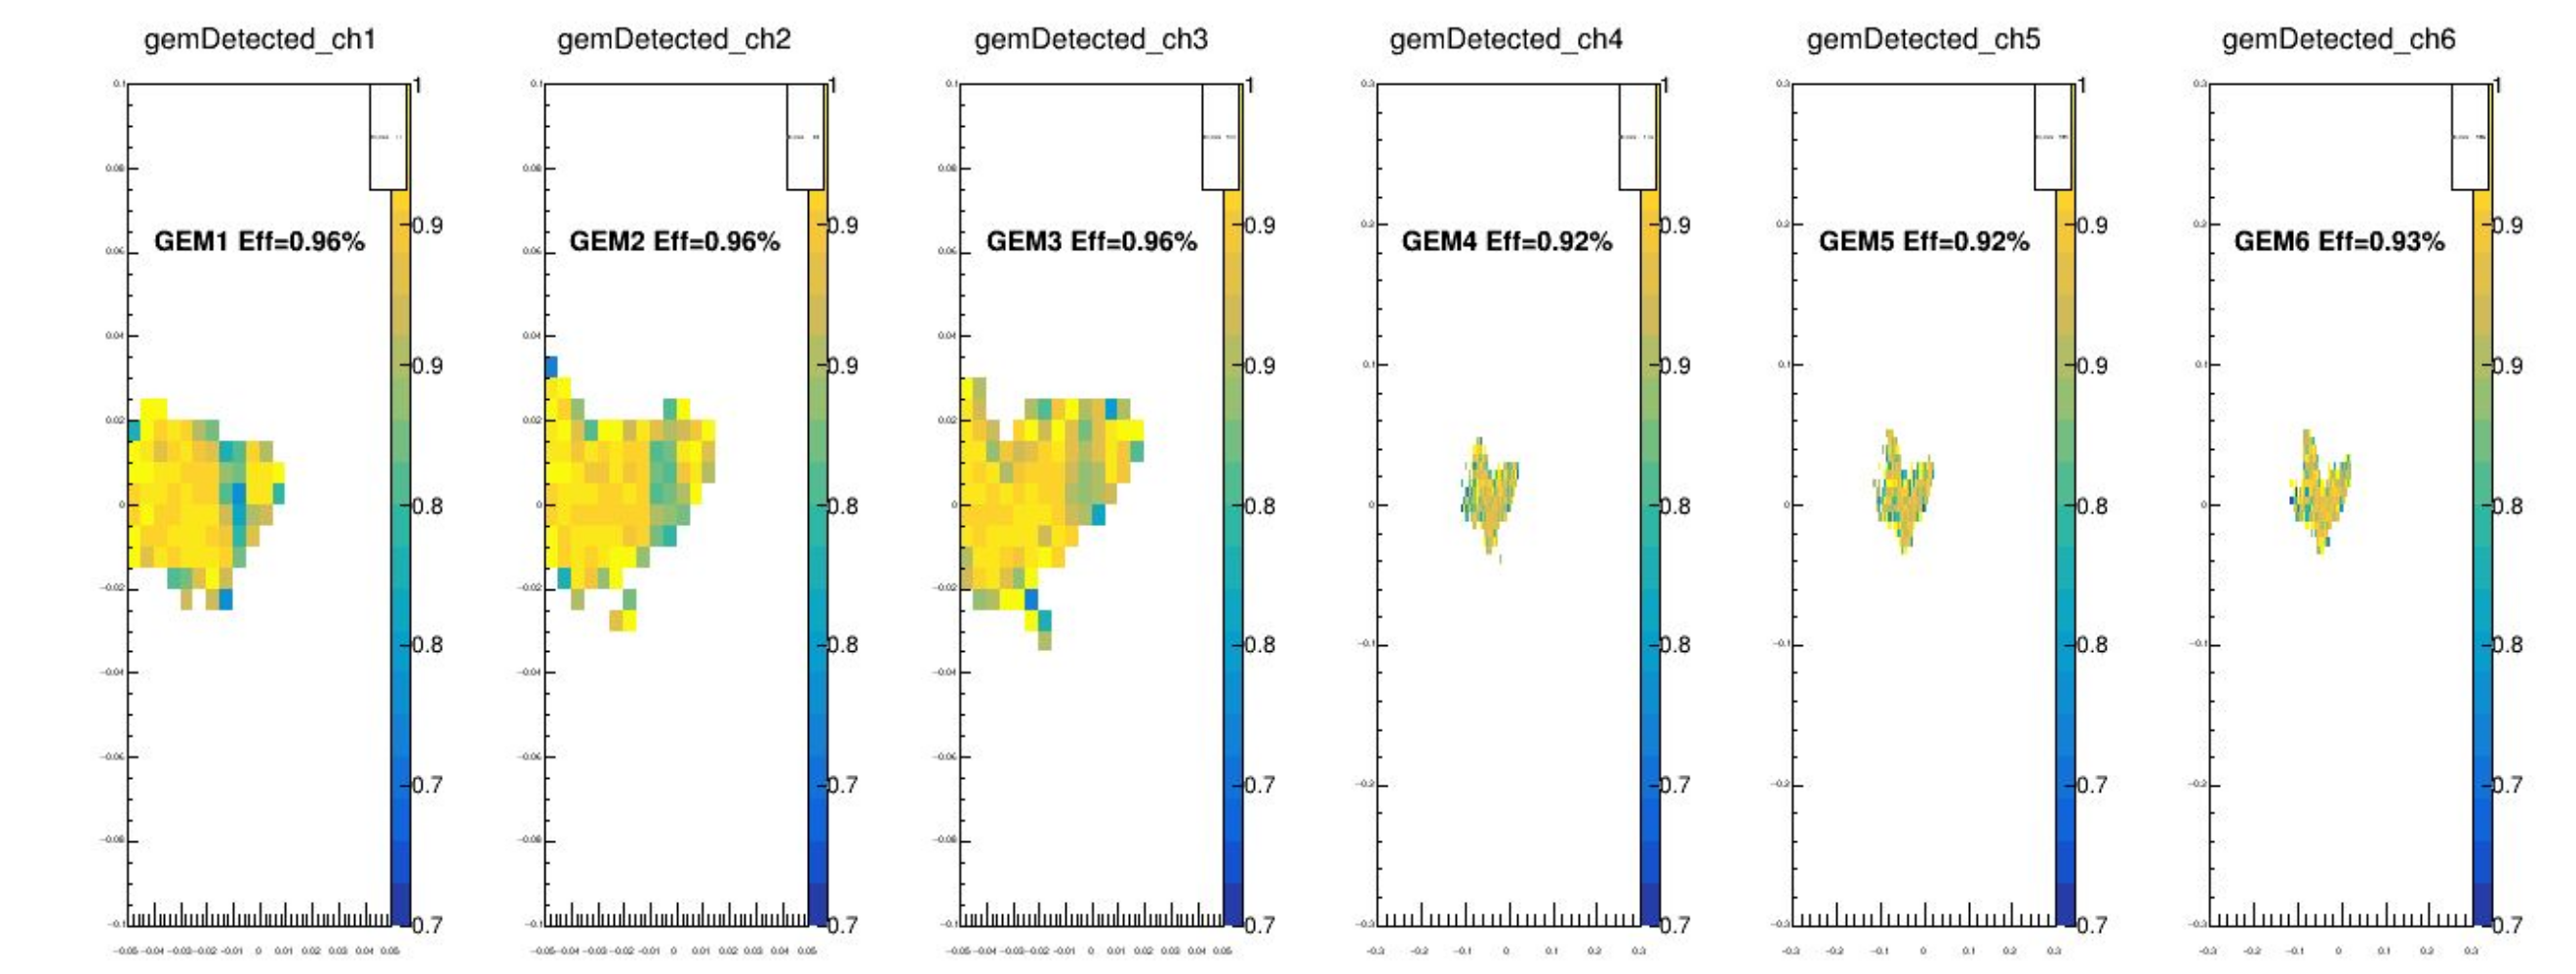
\includegraphics[width=\textwidth]{images/chap5/lhrs_efficiency_2d.png}
    \caption{LHRS GEM detector efficiency}
    \label{fig:lhrs_efficiency_2d}
\end{figure}

\begin{figure}[!htbp]
    \centering
    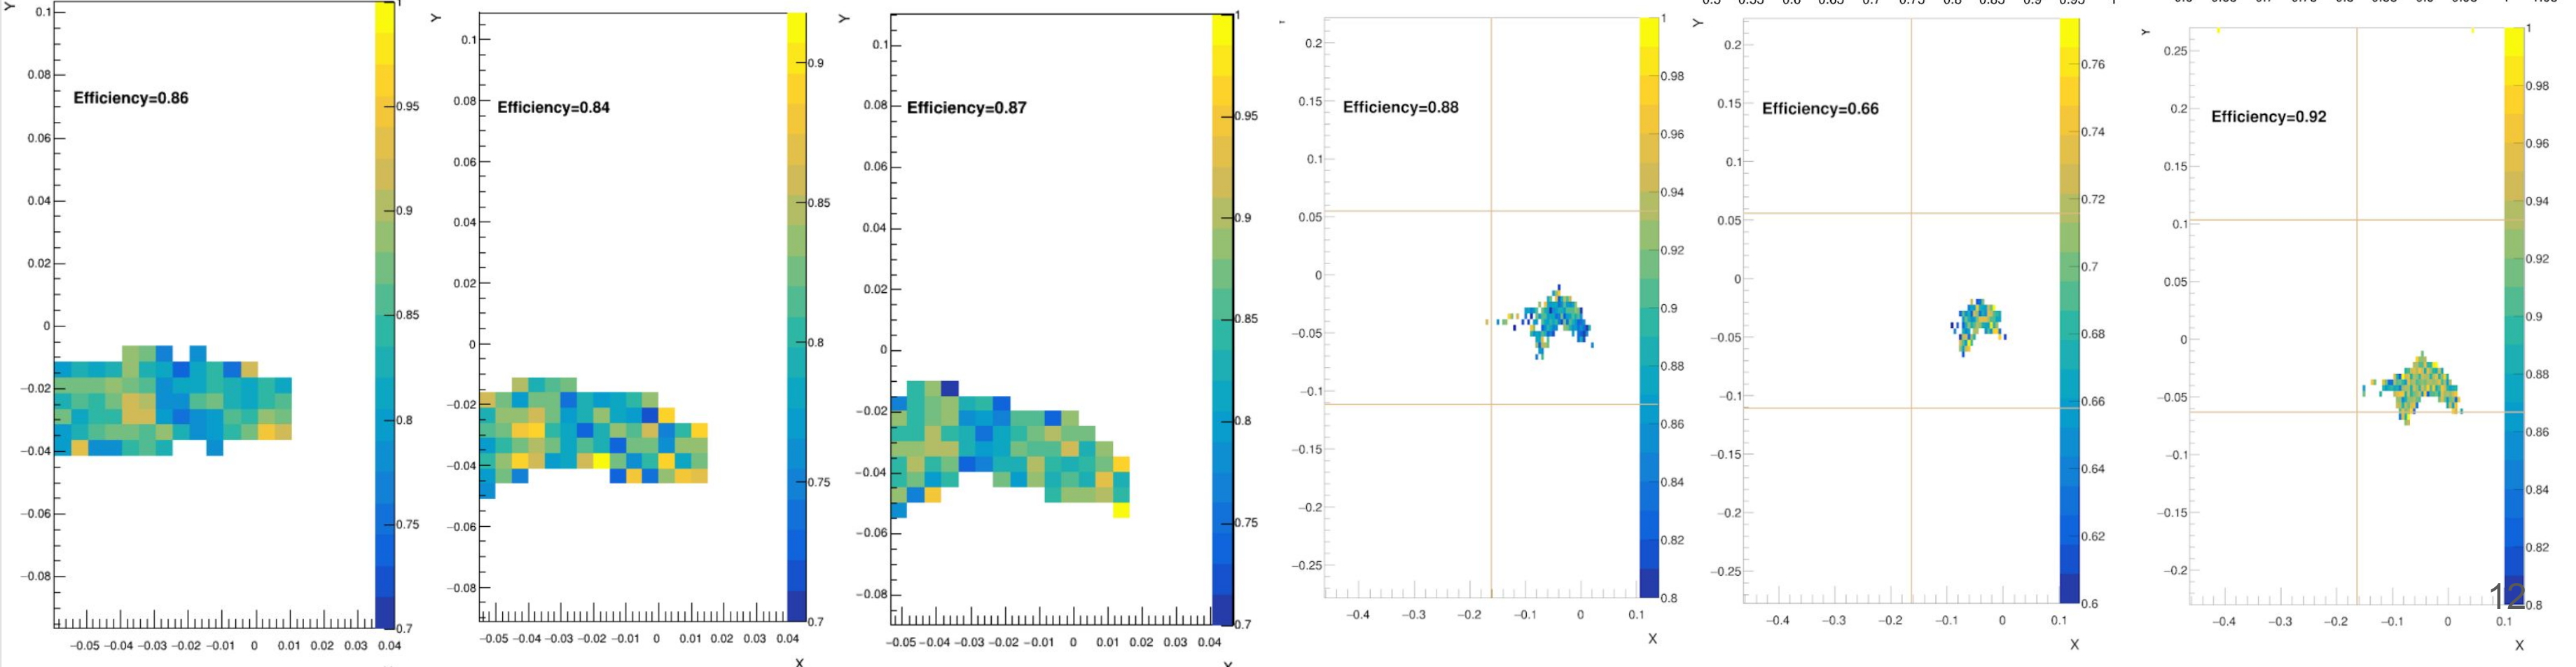
\includegraphics[width=\textwidth]{images/chap5/rhrs_efficiency_2d.png}
    \caption{RHRS GEM detector efficiency}
    \label{fig:rhrs_efficiency_2d}
\end{figure}

To get a better understanding of the efficiency difference by each area, the GEM detector surface area is 
divided into  $1cm \times 1cm$ bins. The efficiency of each bin is computed individually. Figures 
\ref{fig:lhrs_gem_bin_efficiency} and \ref{fig:rhrs_gem_bin_efficiency} show the position dependant 
 efficiency distributions.
\begin{figure}[!htbp]
    \centering
    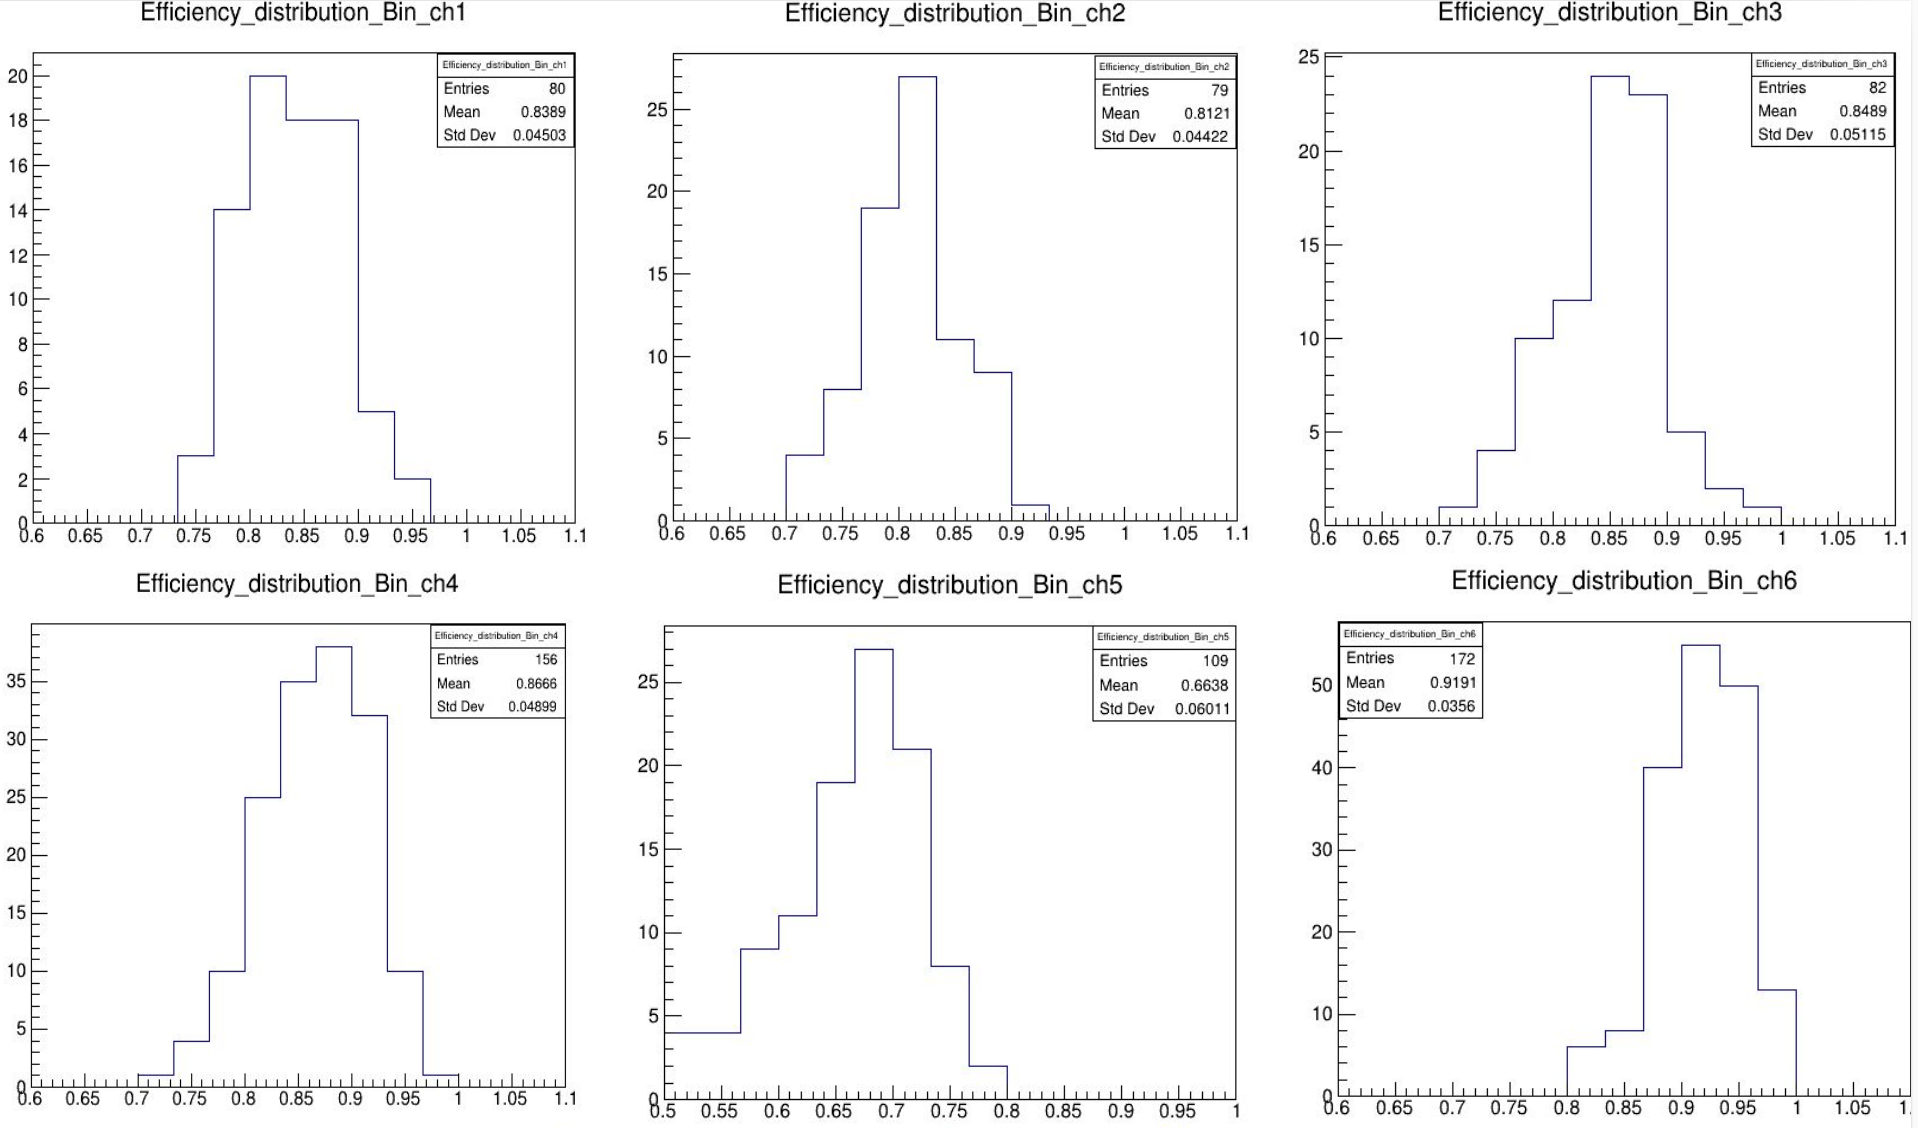
\includegraphics[width=\textwidth]{images/chap5/lhrs_gem_bin_efficiency.png}
    \caption{GEM Efficiency distribution}
    \label{fig:lhrs_gem_bin_efficiency}
\end{figure}

\begin{figure}[!htbp]
    \centering
    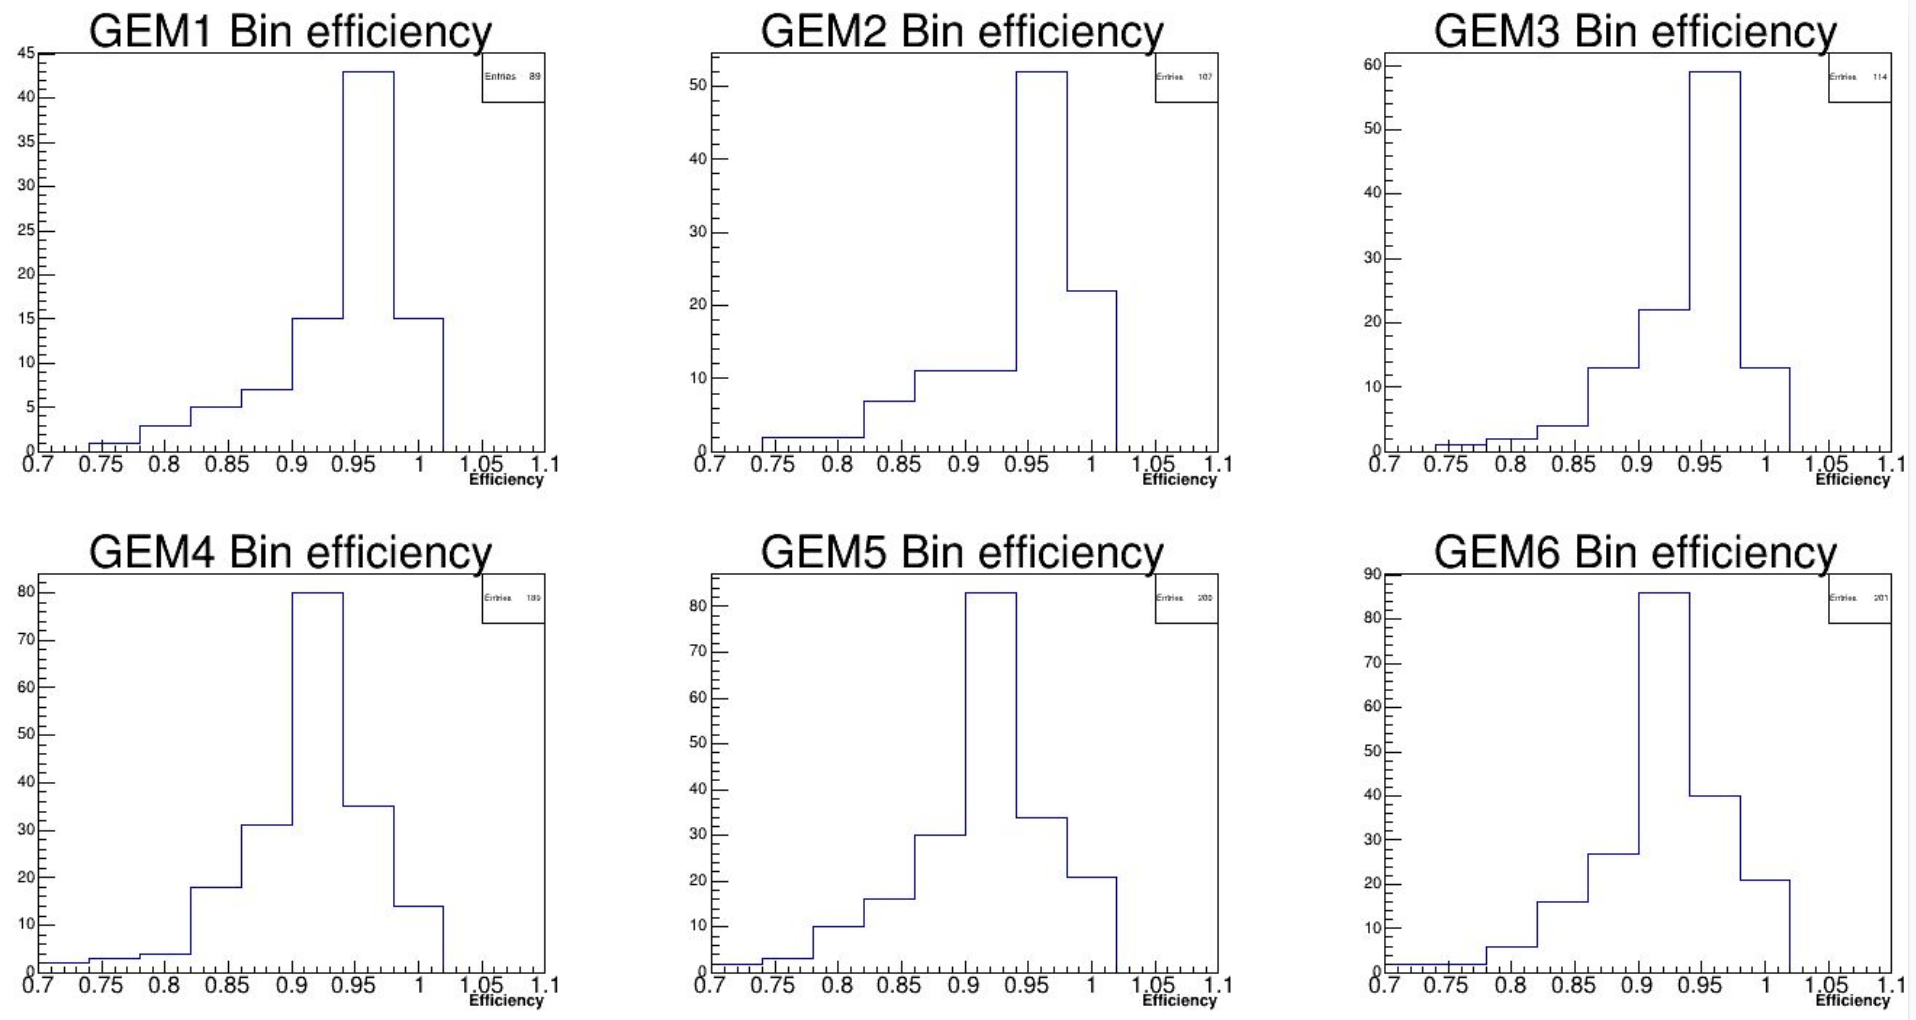
\includegraphics[width=\textwidth]{images/chap5/rhrs_gem_bin_efficiency.png}
    \caption{GEM Efficiency distribution}
    \label{fig:rhrs_gem_bin_efficiency}
\end{figure}

\subsubsection{GEM detector efficiency over time}

GEM detector efficiency increase with time [TO BE ADDED]. 

\subsubsection{GEM detector High Rate Performance and comparison  with VDC}

The GEM detector can achieve a higher event rate than the drift chamber due to its smaller drift time for ions. In the event rate measurement, both GEM and VDC detectors are used for tracking. However, for safety concerns, when the event rate exceeds 500 kHz, only the GEM detector is employed.

Since the VDC detector is not used when the event rate is greater than 500 kHz, a consistent efficiency is obtained by reconstructing the track with six layers of GEM detectors for the efficiency measurement. The VDC efficiency is measured by projecting the GEM track back to the VDC plane and searching for fired events on the VDC detector. Similarly, the GEM efficiency calculation is performed by projecting the track to each GEM detector and searching for fired events in each GEM detector plane.

Figure \ref{fig:apv_25_pedestal_plot} shows the comparison of the GEM detector and VDC detectors at different event rates. The blue points represent the efficiency of the VDC detectors, while the red points represent the efficiency of the GEM detectors. Within the test range from 20 kHz(?) to 1.5 MHz(?), the efficiency of the GEM detector remains consistent. On the other hand, the efficiency of the VDC detector decreases as the event rate increases, dropping to around $60\%(?)$ when the event rate reaches 500 kHz. 

[add all the GEM detectors]



\begin{figure}[!htbp]
    \centering
    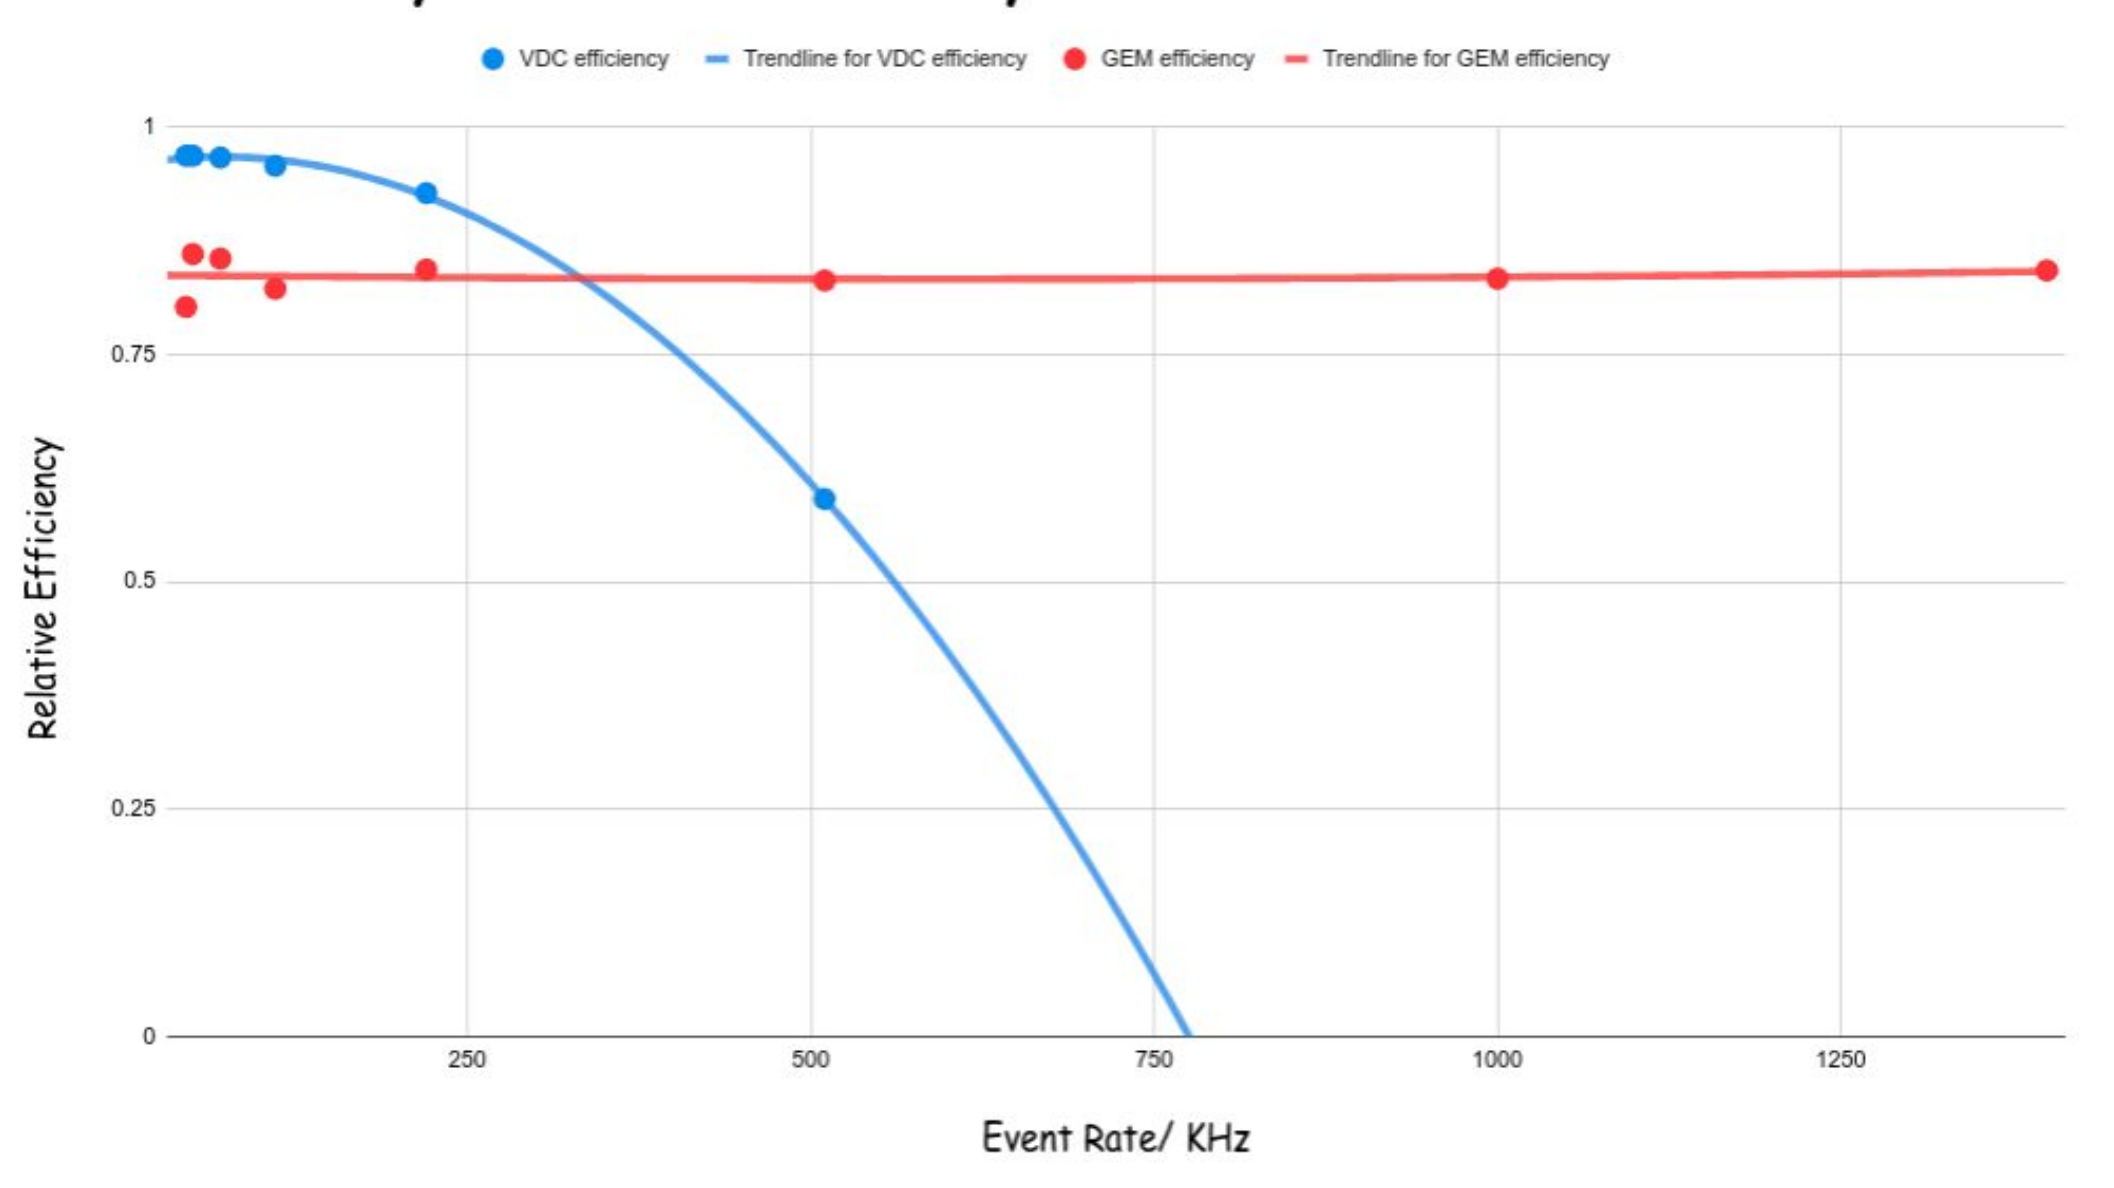
\includegraphics[width=\textwidth]{images/chap5/gem efficiency over time.png}
    \caption{GEM and VDC efficiency Over Time}
    \label{fig:gem_efficiency_over_time}
\end{figure}
